
\subsubsection{Qu'est ce que c'est ?}
On entend souvent dans les médias parler d'intéligence artificielle et de réseaux de neurones,
ces deux notions sont radicalements différentes
mais elles sont souvent mélangées et confondues sur la place publique\ldots \\

L'intéligence artificelle est un concept informatique, un paradigme de programation,
ce n'est pas ce que j'ai fait durant mon stage, on n'en parlera pas ici mais si vous voullez en savoir plus,
je vous redirige vers la chaine youtube de Lê \textsc{Nguyên Hoang}, chercheur en mathématique qui saura
vous l'expliquer bien mieux que moi (à regarder sans moderation)\cite{science4all}. \\

Un réseau de neurones est une architecture informatique permetant de faire
des regressions de fonctions, de la généralisation et de l'optimisation.
Il est composé, comme son nom l'indique, de neurones mis en réseau grace à des connexions.


\subsubsection{Un neurone}
Un neurone (représenté par un cercle dans les schemas) est une unité de base du réseau,
il se decompose en trois phases

\paragraph{L'entrée :}
Un neurone prend des informations en entrée, de manière générale un nombre réel entre 0 et 1
mais d'autres objets sont envisageables (image, pixel, son\ldots).
Il n'y a pas de nombre minimum ou maximums
(on pourait imaginer un neurone ne prenant pas d'entrée, ou au contraire en prenant une infinité),
ni de contrainte sur les differents objets.
\exemle
{
\begin{itemize}
    \item un neurone prenant les trois valleur de coulleur d'un pixel\\
            (entier entre $0$ et $255$).
    \item un neurone prenant les trois valleur de coulleur d'un pixel\\
            (réel $[0, 1]$).
    \item un neurone prenant une sequence \textsc{adn} en entrée

\end{itemize}
}
On note le vecteur entrée $X$ et chacun de ses element $x_1 \ldots x_i \ldots x_n$.

\paragraph{La fonction interne :}
Le réseau vas alors faire un calcul à partir des entrées et de poids,
des valleurs définies pour chaque neurones qui peuvent varier durant l'apprentissage. \\
Le vecteur poid se note $W$ et chacun de ses element $w_1 \ldots w_i \ldots w_n$.

\exemle
{
\begin{itemize}
    \item[$f(X) =$] $W.X = \sum_{i=1}^{n} w_i \times x_i $
    \item[$f(X) =$] $e^{w_1 + x_1} \times w_2$
    \item[$f(X) =$] $\max(X)$
    \item[$f(X) =$] "nombre de A sur les $w_1$ premières bases de $x_1$" \\
            (avec $x_1$ une sequence \textsc{adn})
\end{itemize}
}

\paragraph{La fonction d'activation :}
Comme vus precedement, ces réseaux sont mis en résau,
il est donc interessant d'avoir une norme pour l'entré et la sortie
afin de pouvoir lier des neurones entre eux sans distinctions. \\
La norme qui a été choisie est, comme précedement cité, un réel entre $0$ et $1$.


Or, il peut être remarqué que les fonctions ci dessus ne renvoient pas forcement des nombre entre $0$ et $1$\ldots
On utilise donc la fonction d'activation afin de normaliser les sorties.
\exemle
{
\begin{itemize}
    \item[Pour le cas precedent sur l'\textsc{adn} :] $f(X)/w_1$
    \item[Pour une fonction de $\mathbb{R}$ dans $\mathbb{R}$ :] fonction sigmoide
    \item[Pour une fonction de $\mathbb{R}$ dans $[0, 1 \rbrack$ :] fonction identité
\end{itemize}
}

\paragraph{Pour resumer :}
On prend \textit{des entrées},
on les passe dans la \textit{fonction principale} du neurone,
puis le résultat dans la \textit{fonction d'activation}. \\
Le résultat resemble a cela :
\begin{equation}
    f_{act}(f(X))
\end{equation}
Le tout dépendant bien évidement de $W$ que l'on peut faire varier afin de modifier la fonction du neurone.
\exemle
{
Prenons un neurone avec deux entrées : $x_1$ et $x_2$, \\
de fonction principale $f(X) = X.W$ \\
et de fonction d'activation identité. \\
Si on a $W = (1, 1)$, ce neurone fait une somme.\\
Mais si $W = (0.5, 0.5)$ ce neurone fait une moyenne.
}


\subsubsection{Un réseau}
Une fois que nous avons de nombreux neurones faisant chacuns des actions bien spécifiques,
on voudrais les relier afin de gérer des comportements plus complexes
comme faire une somme de moyenne (ou controller un drone, prédire les mouvements boursiers\ldots).

Il sufit alors de relier les neurones entre eux, de maniere générale de manière linéaire de gauche à droite.
De nombreuse manière de relier les neurones existent (recurent, convolution\ldots),
ici on ne parlera que de la connexion dite "Dense" ou "fully connected" :
le réseau se découpe en $n$ couches de neurones,
chacunes composée de neurones dont les entrées sont les sorties des neurones le la couche précédente.
\begin{figure}[H]
    \center
    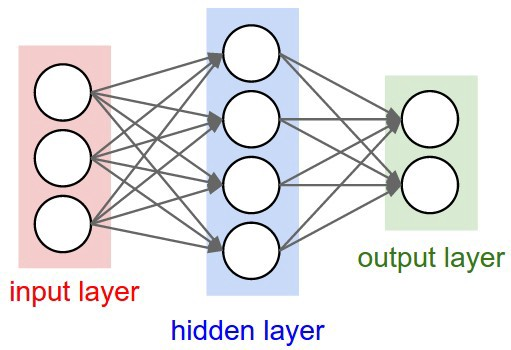
\includegraphics[height=\petit]{pict/net1.jpeg}
	\caption{Réseau dense simple}
	\label{fig:simple-dense}
\end{figure}
Comme on peut le voir sur la figure,
les neurones les plus à gauches sont les neurones d'entrée (capteurs)
et ceux les plus à droite ceux de sortie (controle des moteurs, affichage d'une note\ldots).
Tout les autres neurones sont "cachés", il n'intéragissent pas directement avec l'environement.


\subsubsection{L'apprentissage}
Jusqu'ici on a vus comment creer une architecture modulable permetant d'aproximer toute les fonctions.
Mais une question se pose toujours :\\
Quel est l'intéret ?
Pourquoi ne pas directement écrire la fonction "en dur" ?\\
La réponse tient en trois mots : \textit{Descente de gradient stochastique} (ou  \sgd\ en anglais). \\
Ce concept est ce qui fait que les réseaux de neurones sont les architectures favorites
des data scientists et des chercheurs en \textsc{ia}.\\


L'idée est assez simple, on recherche une fonction générale dont on ne connais que certaines valeurs discretes.
On vas commencer par définir une fonction nomé "loss function"
qui décrit la précision du réseau actuel :
elle prend en entrée deux valeurs : la valeur théorique et la valeur obtenue.
elle retourne un réel positif, plus il est faible, plus le réseau est proche de la fonction théorique.
\exemle
{
\begin{align*}
    loss(exp, obt) = &\ |exp - obt| \\
    loss(exp, obt) = &\ (exp - obt)^2
\end{align*}
}
Le probleme de regression se résume alors à minimiser la fonction de prete,
c'est ici que la descente de gradient stochastique fait son entrée :
Pour minimiser loss, on aimerai bien descendre sa pente, cad dériver suivant les diférentes variables
\footnote{\textsc{NB :} Ici les variables sur lesquels on intervient sont les $w_i$ (pas les $x_i$).}.
Étant donné que de manière générale, il y a plusieurs variables, la dérivée se transforme en gradient.
Ainsi, afin de pouvoir calculer facilement les gradients,
des applications linéaires sont privilégiées dans les fonctions des neurones.\\


On a donc expliqué d'ou vient la descente de gradient, mais que veut dire stochastique ?
Le mot stochastique est synonyme de hasard.
En effet le temps de calcul du gradient est exponentiel
alors lorsque le réseau est grand
(un réseau peut facillement atteindre le million de neurones voir même des milliards\cite{i3espectrum})
il est inimaginable de calculer la totalité du gradient, on utilise alors le gradient stochastique.\\


Cette descente de gradient est extremement rapide, ainsi, il est possible de l'iterer de nombreuses fois
pour essayer de minimiser la fonction de perte.
L'espaces des solutions étant rarement idéal
(rarement une "cuvette" mais constitué de "bosses" et de "trous" chaotiques)
il n'est pas obligatoire d'arriver à atteindre le minimum global mais au moins minimum local sera atteind.
Ainsi, avec plusieurs apprentissages on peut approximer très efficacement quasiment toutes les fonctions.
